s
This section documents the results on the $\WW$ cross-section measurement. 
The selections are the same as in the $\WW$ preselection defined in 
Section~\ref{sec:selection}, except for the following two differences

\begin{enumerate}
\item {The trailing lepton threshold is 20 \GeV}
\item {The $\met$ selections used are from the high mass Higgs strategy}
\end{enumerate}


\subsection{Background  Estimations}

The background estimations use the same method as in the Higgs search 
documented in Section~\ref{sec:backgrounds}.

The Drell-Yan background estimation is tabulated in Table~\ref{tab:dy_wwxsec}. And the 
Top background estimation is tablulated in Table~\ref{tab:top_wwsec}. 
%%%%%%%%%%%%%%%%%%%%%%%%%%%%%
\begin{table}[!hbtp]
\begin{center}
\begin{tabular}{l|cccc}
\hline
Final State & $N(\ell\ell)_{\textrm{control}}^{\textrm{data}}$  & $N_{\textrm{control}}^{\textrm{ZV, sim.}}$ & $R_{out/in}$ & $N_{out}$ (data) \\ 
\hline
ee                          & 26   & $9.3 \pm 0.2 \pm 0.9$       & $0.23 \pm 0.12 \pm 0.06$    & $2.8 \pm 1.9 \pm 0.8$  \\
$\mu\mu$                    & 40   & $13.5 \pm 0.2 \pm 1.4$       & $0.19 \pm 0.07 \pm 0.03$    & $3.6 \pm 1.9 \pm 0.6$ \\
$e\mu$                      & 12    & -                             & -                         & -\\ 
\hline
$ee$ and $\mu\mu$ combined  & 76   & $22.8 \pm 0.3 \pm 2.3$     & $0.21 \pm 0.06 \pm 0.02$    & $6.3 \pm 2.7 \pm 0.8$ \\
\hline
\end{tabular}
\end{center}
\caption{ Predictions of the off-peak $Z/\gamma^*$ contribution 
for events passing all $WW$ selections. Both statistical and systematic uncertainties 
are displayed. For the $VZ$ contribution in the control region, we assign 10\% systematics due to the 
uncertainty in the cross-sections. }
\label{tab:dy_wwxsec}
\end{table}
%%%%%%%%%%%%%%%%%%%%%%%%%%%%%%

%%%%%%%%%%%%%%%%%%%%%%
\begin{figure}[!hbtp]
\centering
\subfigure[ee]{
\centering
\label{subfig:dyr_ee_0j}
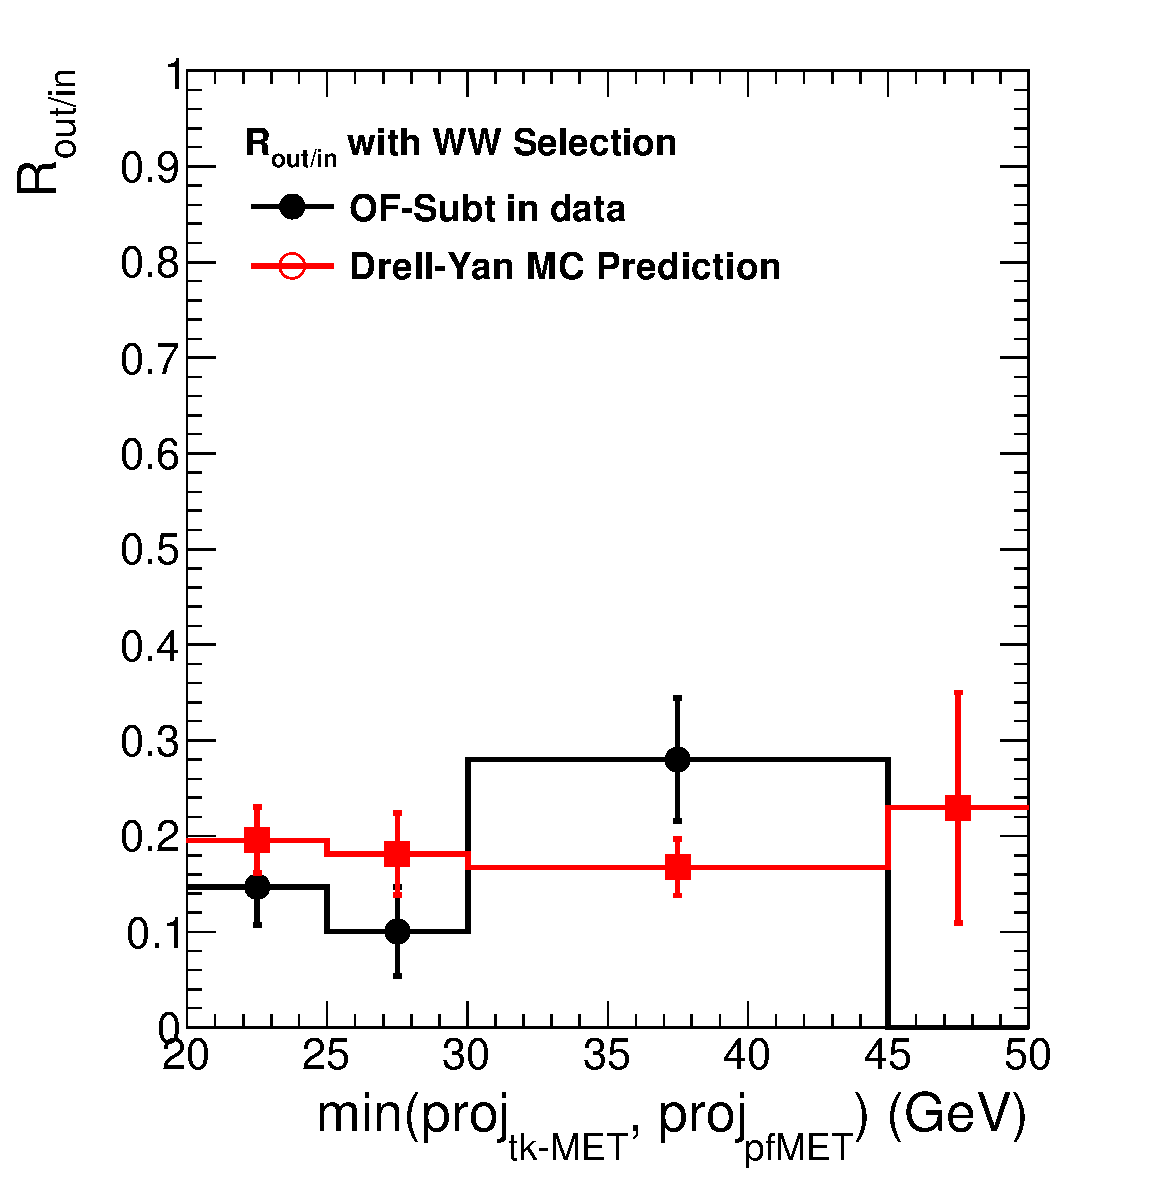
\includegraphics[width=.3\textwidth]{figures/Routin_ee_0Jet_mH0_818pb_dy.pdf}}
\subfigure[mm]{
\centering
\label{subfig:dyr_mm_0j}
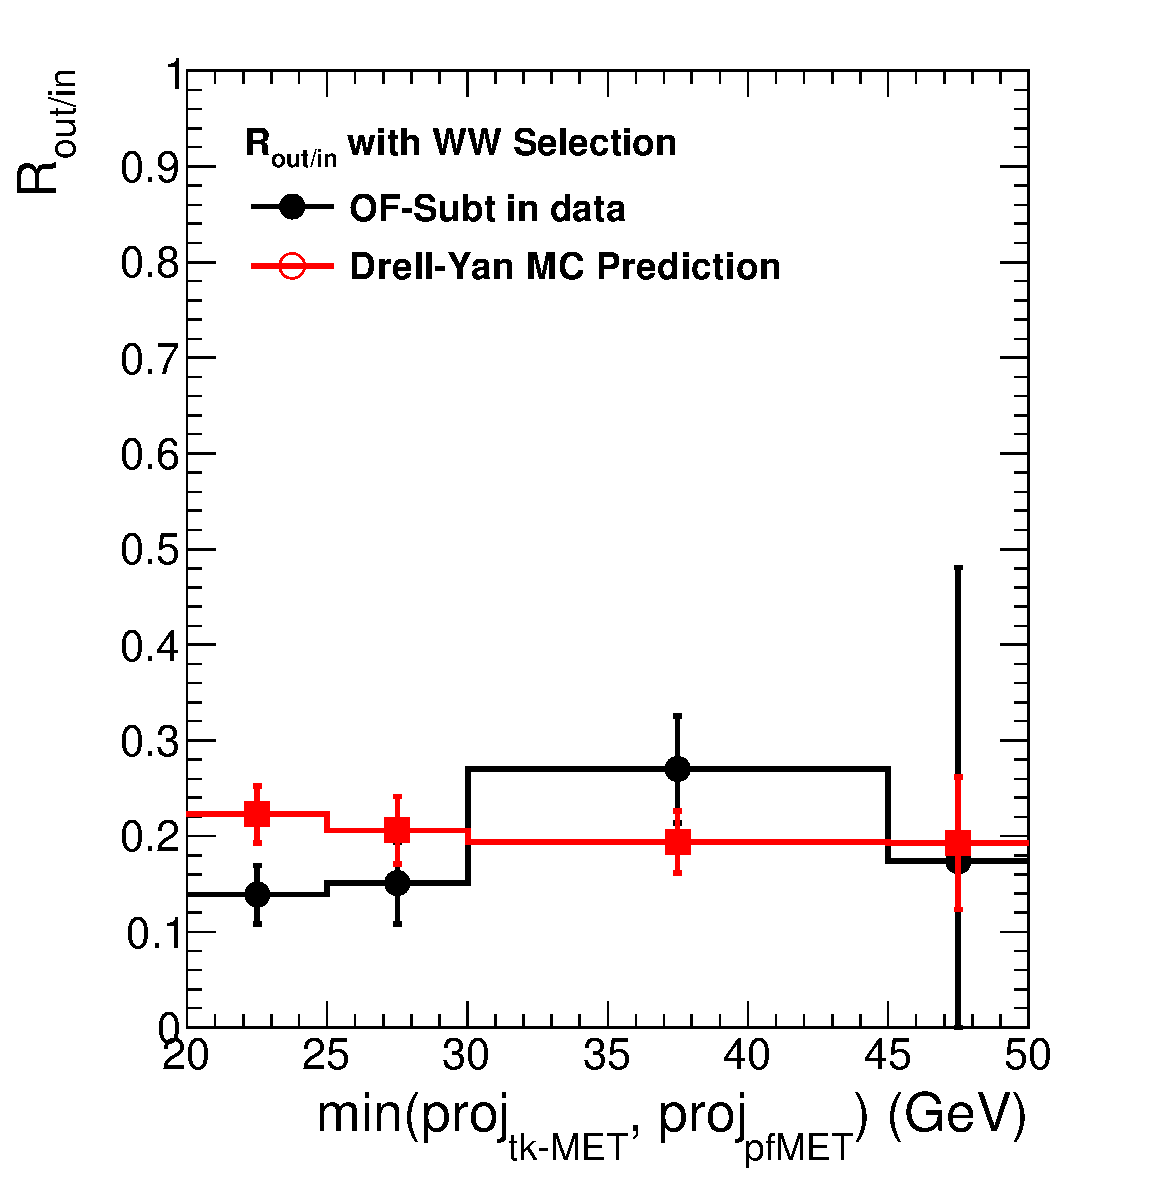
\includegraphics[width=.3\textwidth]{figures/Routin_mm_0Jet_mH0_818pb_dy.pdf}}
\subfigure[ee/mm combined]{
\centering
\label{subfig:dyr_ll_0j}
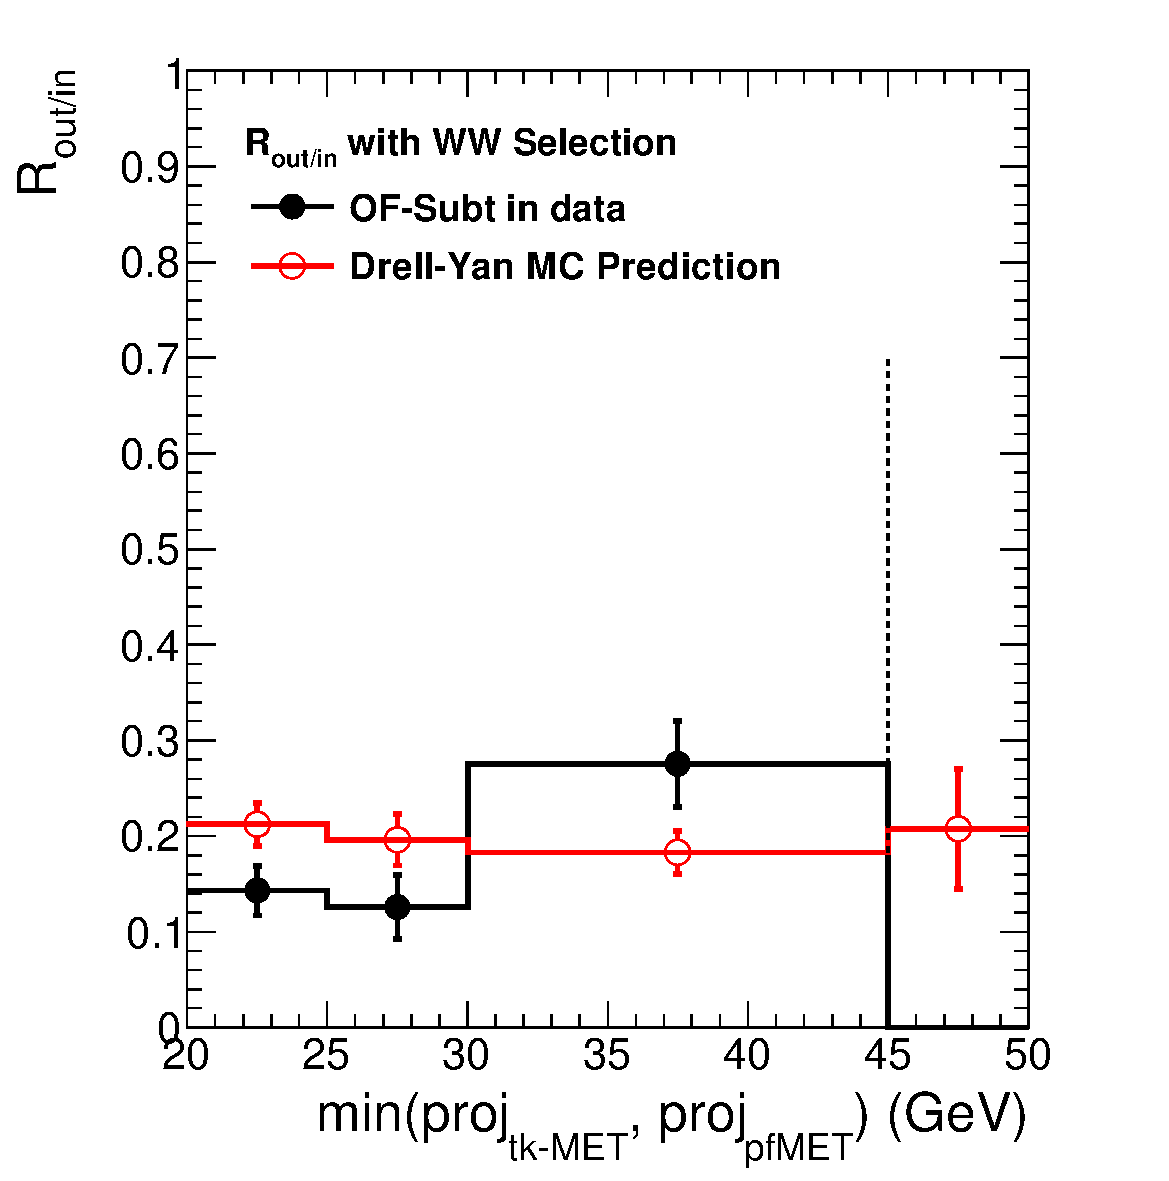
\includegraphics[width=.3\textwidth]{figures/Routin_0Jet_mH0_818pb_dy.pdf}}
\caption{
 The \routin\, as a function of MET measured from data (black solid dots) 
and MC (red open circles) for the Drell-Yan processes. The measurements 
in data are done using the opposite flavor subtraction method, with the 
last bin blinded in data. }
\label{fig:dyr_ww}
\end{figure}
%%%%%%%%%%%%%%%%%%%%%%

%%%%%%%%%%%%%%%%%%%%%%%%%%%%%% 
\begin{table}[ht!]
\begin{center} 
\begin{tabular}{l c}
\hline
                             Parameter      & Value             \\
\hline
       Estimated top events in simulation   & 27.9  $\pm$ 1.6   \\
                   tagging efficiency (\%)  & 57.3  $\pm$ 4.5   \\
                top-tagged events in data   & 40             \\
      background events in control region   & 7.8  $\pm$ 2.4  \\
      Data-driven top background estimate   & 24.0 $\pm$ 6.7  \\
                            Scale factors   & 0.86  $\pm$ 0.24  \\
\hline
\end{tabular}  
\caption{Monte Carlo to data scale factor for the top background contribution for $\intlumiEightTeV$.}  
\label{tab:top_wwsec}
\end{center}
\end{table}
%%%%%%%%%%%%%%%%%%%%%%%%%%%%%%



\subsection{Cross-section Measurement}

We now calculate the $\WW$ production cross section according to equation \ref{eq:mainformula},

\begin{equation}
\label{eq:mainformula}
\sigma_{WW}  = \frac{N_{data} - N_{bkg}}{\epsilon \cdot {\cal{L}} \cdot BR(WW \to \ell \nu \ell \nu)}
\end{equation}

Where $N_{data}$ is the number of events observed in data, $N_{bkg}$ is the estimated number
of background events, which are summarised with their uncertainties in Table \ref{tab:data_yields}.
The distributions of the $p_{T}$ of the leading and trailing leptons, and the dilepton $p_{T}$ 
and invariant mass are shown in Figure \ref{fig:inclplots}.
The efficiency to select $\sigma_{WW \to 2\ell 2\nu}$
candidates, $\varepsilon$, is computed as the weighted mean of
the $qq\to\WW$ and $gg\to\WW$ efficiencies in simulation.
Assuming a 3\% contribution from the $gg$ process, 
$\varepsilon$ is found to be $(3.38 \pm 0.28)\%$.
The integrated luminosity of the data sample is ${\cal{L}} = $ 4920 $\pm$ 108 $\ipb$, 
and the branching ratio $BR(WW \to \ell \nu) =$ 0.1080 $\pm$ 0.0009~\cite{pdg}.

\begin{table}[ht!]
  \begin{center}
  \begin{tabular} {|c|c|}
\hline
Sample                & Yield $\pm$ stat $\pm$ syst \\ \hline \hline
$qqWW$                & 148.2 $\pm$  1.2 $\pm$ x.x  \\ \hline
$ggWW$                & 10.0 $\pm$  0.2 $\pm$ x.x  \\ \hline
$t\bar{t} + tW$       & 24.0 $\pm$  1.4 $\pm$ 6.8  \\ \hline
$W+jets$              & 13.1 $\pm$  2.6 $\pm$ 4.6  \\ \hline
$WZ$                  & 4.9 $\pm$  0.2 $\pm$ 0.5  \\ \hline
$ZZ$                  & 1.8 $\pm$  0.1 $\pm$  0.2  \\ \hline
$Z/\gamma*$           & 6.3 $\pm$  2.7 $\pm$  0.8  \\ \hline
$W\gamma*/W+\gamma$   & -    \\ \hline \hline
Total Bkgd.           & 208.6 $\pm$  3.6 $\pm$ x.x  \\ \hline \hline
%Total Bkgd.+Signal    & 1061.1 $\pm$  7.8 $\pm$ 62.0  \\ \hline \hline
Data                  & 246 \\ \hline
\end{tabular}
  \caption{Expected number of signal and background events from the data-driven methods for
  an integrated luminosity of \intlumiEightTeV after applying the selection requirements 
in the $\mu\mu$, $\mu{e}$, $e\mu$ and $ee$  channels.}
   \label{tab:data_yields}
  \end{center}
\end{table}

%%%%%%%%
\begin{figure}[!hbtp]
\begin{center}
\subfigure[Leading lepton $p_{T}$]{\label{subfig:fig_inclplots_pt1}
%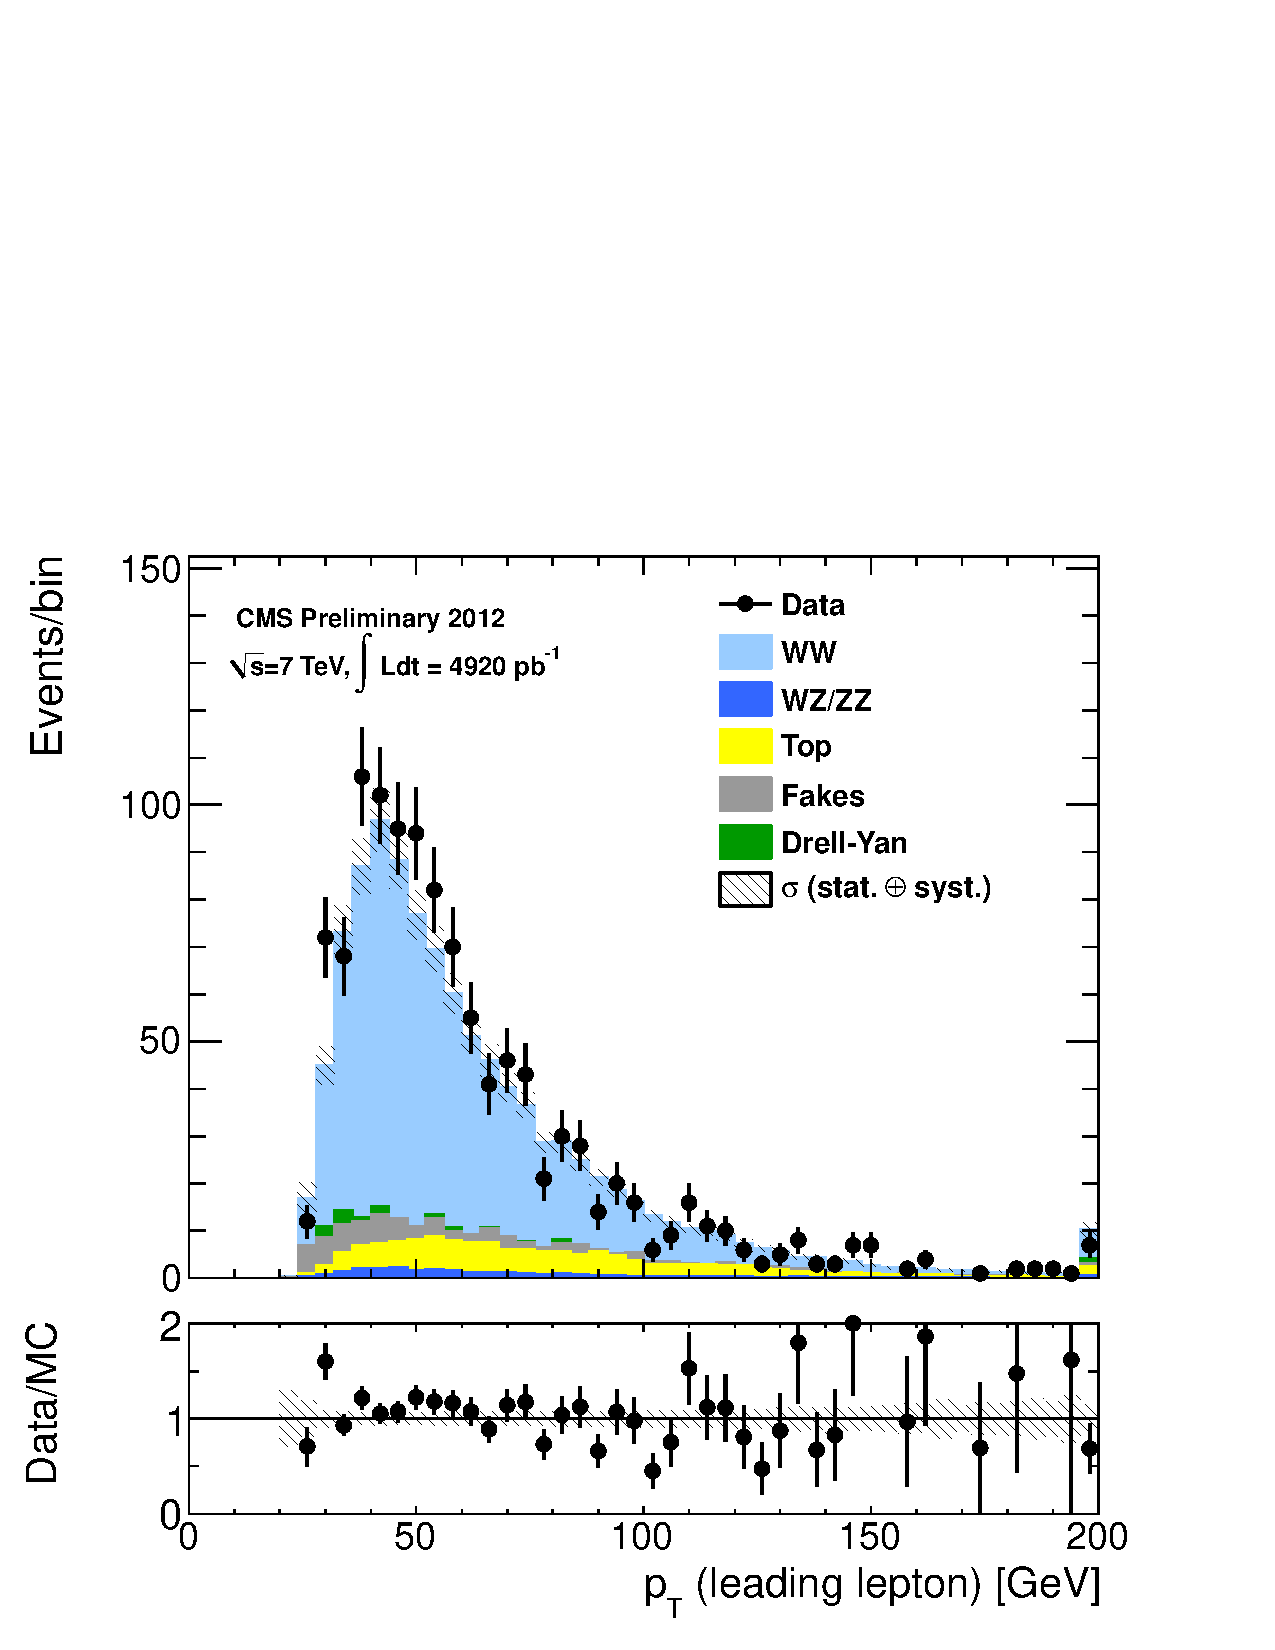
\includegraphics[width=.45\textwidth]{figures/pas_pt1_incl.pdf}
}
\subfigure[Trailing lepton $p_{T}$]{\label{subfig:fig_inclplots_pt2}
%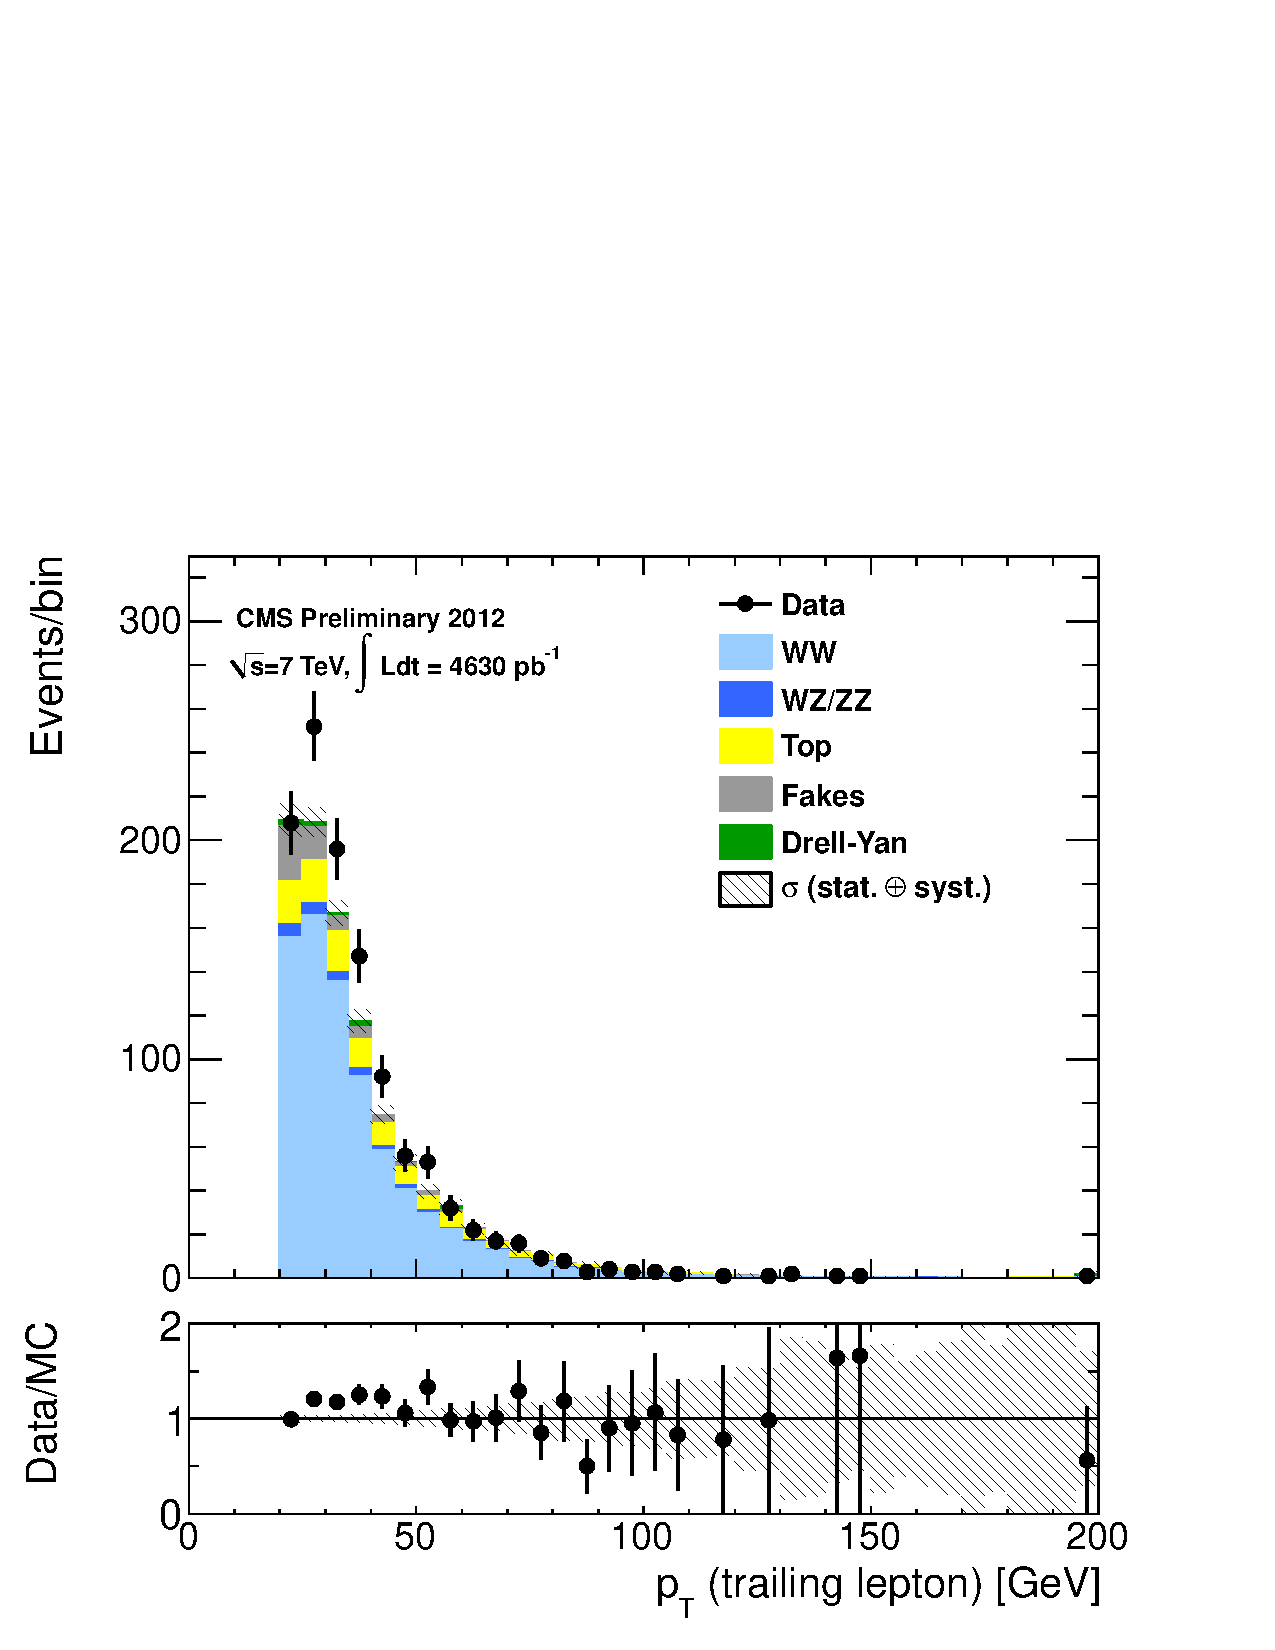
\includegraphics[width=.45\textwidth]{figures/pas_pt2_incl.pdf}
}
\subfigure[Dilepton system $p_{T}$]{\label{subfig:fig_inclplots_ptll}
%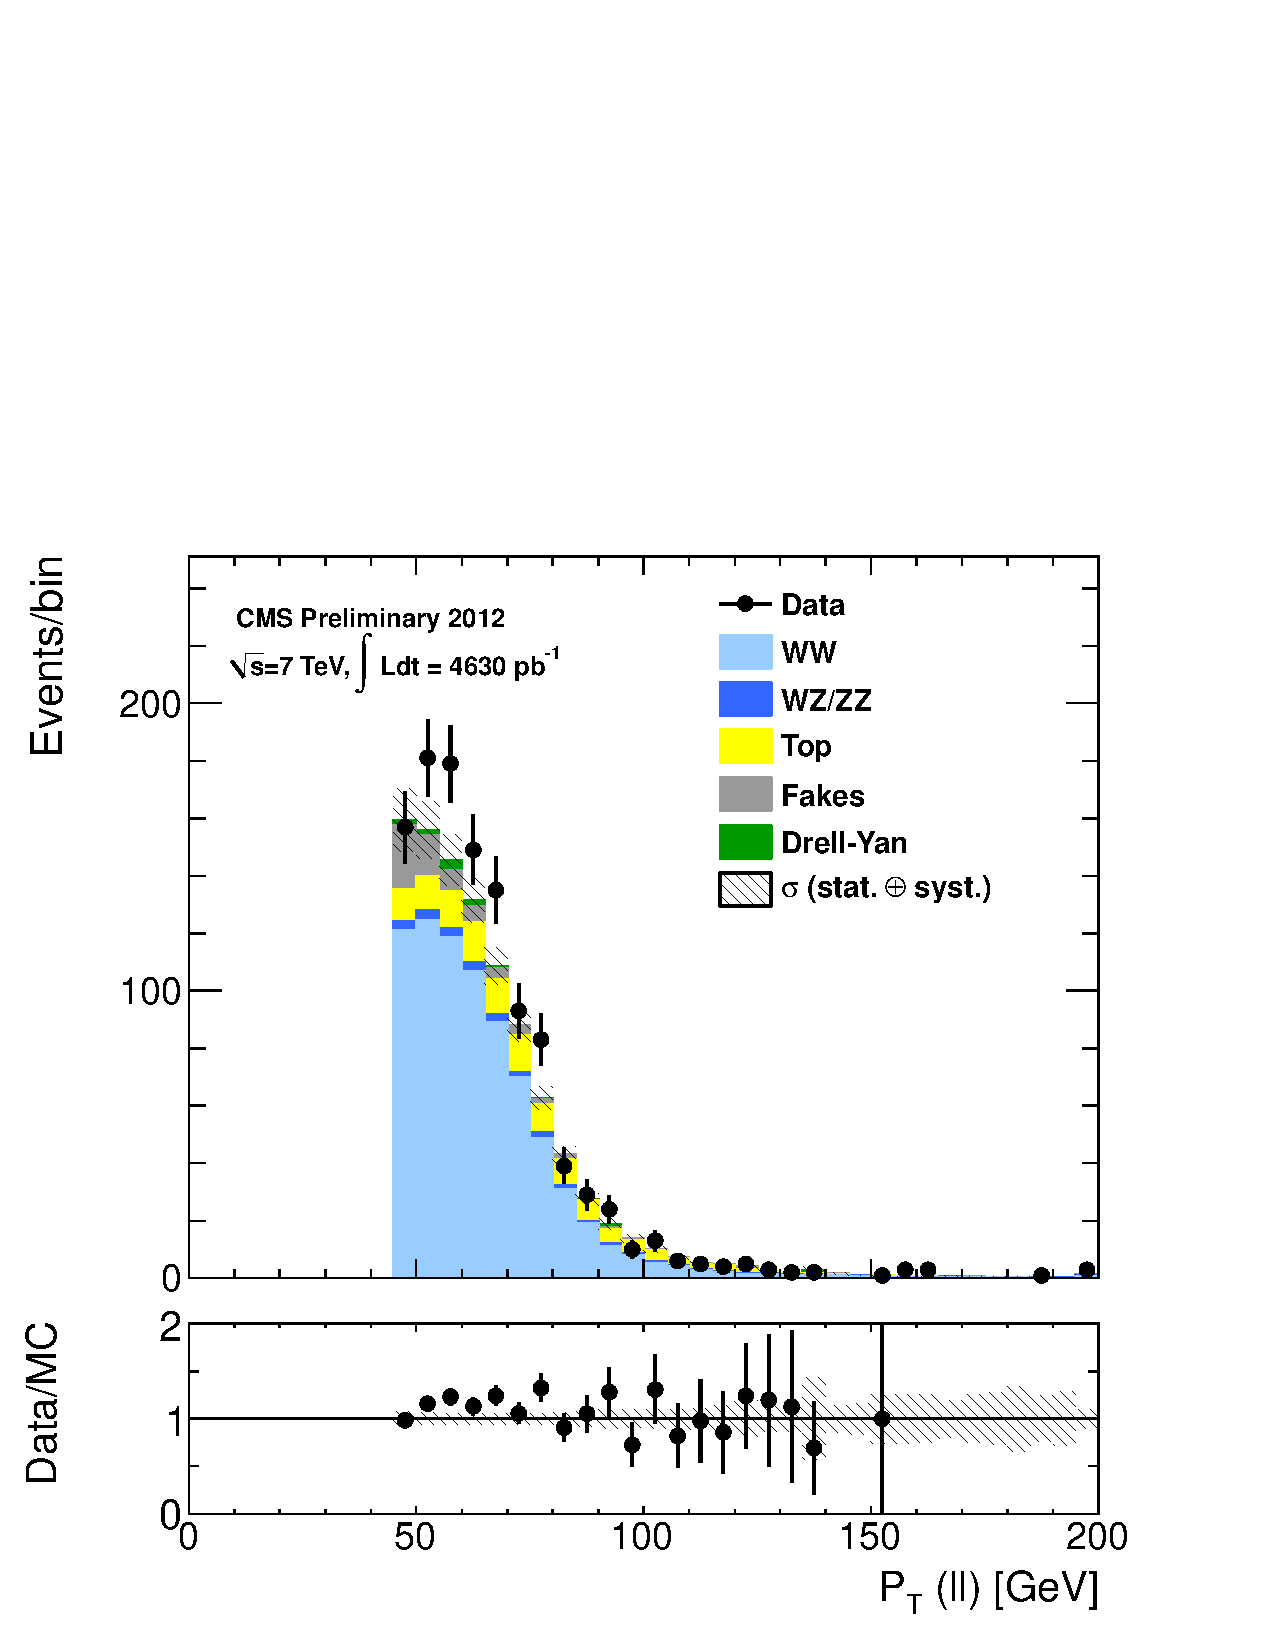
\includegraphics[width=.45\textwidth]{figures/pas_ptll_incl.pdf}
}
\subfigure[Dilepton system invariant mass]{\label{subfig:fig_inclplots_M}
%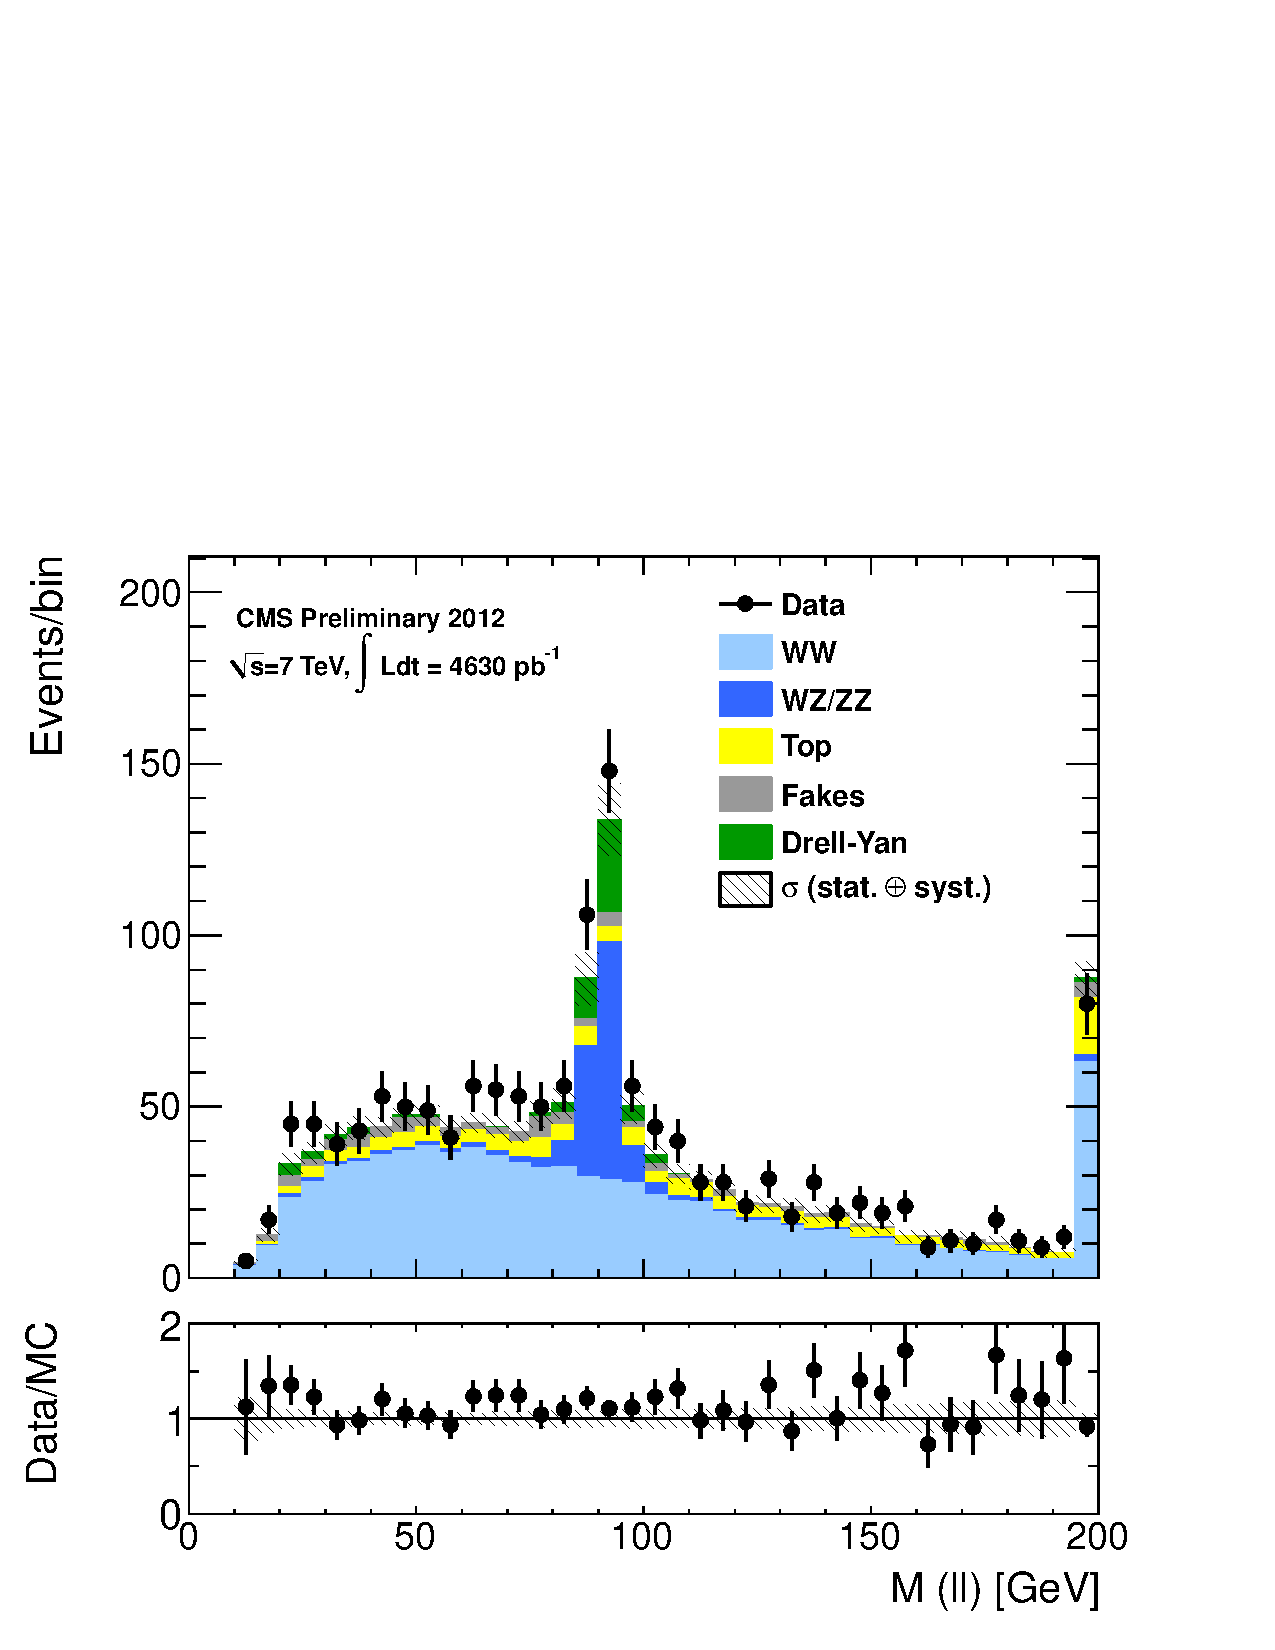
\includegraphics[width=.45\textwidth]{figures/pas_mll_incl.pdf}
}
\caption{Kinematic distributions for expected and observed events in the  $\mu\mu$, $\mu{e}$, $e\mu$ and $ee$ channels.
The dilepton system invariant mass distribution has the $Z$ mass veto relaxed.
The uncertainty on the expected events includes both statistical and systematic components.}
\label{fig:inclplots}
\end{center}
\end{figure}
%%%%%%%%


Using the inputs described previously and Equation \ref{eq:mainformula},
we obtain the following $WW$ cross-section measurement:

\begin{equation*}
\sigma_{WW}  = X \pm X ~\mathrm{(stat.)} \pm X ~\mathrm{(syst.)} \pm X ~\mathrm{(lumi.)~pb}.
\end{equation*}

%The cross section obtained in each dilepton channel is documented in Appendix \ref{sec:xsec_per_channel}.

